\documentclass[conference]{IEEEtran}
\IEEEoverridecommandlockouts
% The preceding line is only needed to identify funding in the first footnote. If that is unneeded, please comment it out.
\usepackage{cite}
\usepackage{amsmath,amssymb,amsfonts}
\usepackage{graphicx}
\usepackage{textcomp}
\usepackage{xcolor}
\usepackage{ifpdf}
\usepackage{epsfig,graphicx}
\usepackage{float}
\usepackage{algorithm,algorithmic}
\usepackage{microtype}
\usepackage{mathtools}
\usepackage{amssymb,amsmath,epsfig, graphics,floatflt}
\usepackage{comment}
\pagestyle{empty}
\usepackage{amsmath}
\usepackage{subfigure}
\usepackage{array}
\usepackage{fixltx2e}
\usepackage{subcaption}
\usepackage[labelformat=parens,labelsep=quad,skip=3pt]{caption}
\usepackage{url}
\def\BibTeX{{\rm B\kern-.05em{\sc i\kern-.025em b}\kern-.08em
    T\kern-.1667em\lower.7ex\hbox{E}\kern-.125emX}}
\begin{document}

\title{Design and Development of Drone Seed Dispersal Mechanism using Novel Narcondam Hornbill Algorithm in Barren Lands}
 
\author{	\IEEEauthorblockN{Suresh Chavhan \IEEEauthorrefmark{1}, Beerelly Srinitha \IEEEauthorrefmark{1}, Sikander Kathat \IEEEauthorrefmark{1}, Ashit Kumar Dutta \IEEEauthorrefmark{2}, Joel J. P. C. Rodrigues\IEEEauthorrefmark{3}\\	}

\vspace{0.1in}
\IEEEauthorblockA{\IEEEauthorrefmark{1}Department of Computer Science and Engineering,\\ Indian Institute of Information and Technology Raichur, Karnataka, India.\\
\IEEEauthorrefmark{2} Department of Computer Science and Information Systems, College of Applied Sciences,\\ AlMaarefa University, Ad Diriyah, Riyadh, 13713, Kingdom of Saudi Arabia.\\ 
\IEEEauthorrefmark{3} Amazonas State University, Manaus - AM, Brazil.\\ }
(E-mail: suresh@iiitr.ac.in, srinithabeerelly1905@gmail.com,  sikanderkat@gmail.com, adotta@um.edu.sa, joeljr@ieee.org)}

\maketitle

\begin{abstract}
Seed dispersal plays a crucial role in the survival of plant species, but human activities are disrupting this process, leading to ecosystem degradation. There is a need to develop innovative seed dispersal algorithms to restore degraded ecosystems and prevent further biodiversity loss. Drones can be used as powerful tools to assess the state of ecosystems, identify areas requiring seed dispersal, and monitor restoration progress. By leveraging drones, more effective seed dispersal algorithms can be developed to promote diverse plant communities and ensure long-term ecosystem sustainability. One of the challenges in simulating seed dispersal is the difficulty in accounting for the complex interactions between different environmental factors and seed characteristics. The proposed algorithm aims to address existing models' limitations and improve seed dispersal efforts' effectiveness. This algorithm utilizes the endozoochory process of the Narcondam Hornbill to optimize seed dispersal efficiency, which has been successfully tested and implemented in simulated environments.
\end{abstract}

\begin{IEEEkeywords}
Narcondam Hornbill, Drone, Seed Balls, Dropping Mechanism, Seed Dispersal
\end{IEEEkeywords}
%\section*{Abstract}

\section{Introduction}
Seed dispersal is a crucial process that contributes to the survival and diversity of plant species. In nature, seed dispersal is carried out by a variety of mechanisms such as wind, water, animals, and birds. Among these, avian seed dispersal, or ornithochory, is considered to be one of the most effective methods for seed distribution, as birds can cover large areas quickly and disperse seeds over a range of habitats. The efficient and effective dispersal of seeds is essential for the survival and regeneration of many plant species, but anthropogenic factors are increasingly disrupting this process, leading to biodiversity loss and ecosystem decline. In the absence of scalable and practical solutions, up to 95\% of the world's ecosystems could be impacted by seed dispersal degradation by 2050. Therefore, there is an urgent need to develop and implement innovative seed dispersal algorithms to restore degraded ecosystems\cite{1} and stem biodiversity loss. To achieve this, the most advanced and efficient tools are required, which include unmanned aerial vehicles, or drones. 
\\Drones have proven to be valuable tools in various sectors, such as environmental conservation, forestry, and agriculture\cite{2}. However, their use in restoration ecology for seed dispersal has been limited so far. Therefore, this article aims to highlight the potential uses of drones in seed dispersal algorithms for ecological restoration. Drones can accurately assess the state of ecosystems, identify areas that require seed dispersal, and monitor the progress of the restoration process over time\cite{3}. With the help of drones, more effective seed dispersal algorithms can be developed to promote the growth of diverse plant communities and ensure the long-term sustainability of ecosystems. In recent years, computer scientists have developed various algorithms for simulating seed dispersal and optimizing the process for real-world applications. However, many of these algorithms are limited in their efficiency and accuracy and do not fully capture the complexity of the natural processes of seed dispersal. The Narcondam Hornbill can serve as an important source of inspiration for developing more effective seed dispersal algorithms and highlights the potential of avian seed dispersal for restoring and maintaining biodiversity in natural ecosystems. This contributes to the growing body of knowledge on the role of birds in ecosystem functioning and emphasizes the need for innovative and sustainable solutions to address the global challenge of seed dispersal in barren lands.
\\A new seed dispersal algorithm inspired by the endozoochory process of the Narcondam Hornbill\cite{4} is presented. The Narcondam Hornbill is a bird found only on the remote island of Narcondam in the Andaman and Nicobar archipelago and plays a critical role in the seed dispersal of many plant species. By consuming fruits and seeds, the bird helps to transport them to new locations, where they can germinate and grow. The algorithm is designed to simulate the endozoochory process of the Narcondam Hornbill and to optimize seed dispersal for real-world applications. The various components of the algorithm, including the selection of suitable plant species, the design of the seed mixture, and the simulation of bird movement patterns are discussed.

The rest of the paper is organized as follows. Section II comprehensively presents the Narcondam hornbill. Section III presents a proposed Narcondam hornbill system architecture. Section IV discusses the proposed Narcondam Hornbill algorithm. Section V shows the simulation scenario, dataset, results, and analysis. Finally, conclusions and future works are drawn in Section VI.
\section{Overview of Narcondam Hornbill}
The Narcondam Hornbill (Rhyticeros narcondami) is a bird species found only on the small island of Narcondam\cite{5} in the Andaman and Nicobar archipelago of India. It plays an important role in seed dispersal on the island. The Narcondam Hornbill feeds on a variety of fruits, including figs, guavas, and other fleshy fruits. As the bird consumes the fruit, the seeds pass through its digestive system and are deposited in its droppings in different locations across the island. This process of seed dispersal through ingestion by birds is called endozoochory. The seeds in the hornbill's droppings have a better chance of germination and growth because they have been partially digested and their hard outer shells have been broken down, making it easier for the young plant to emerge. Overall, the Narcondam Hornbill is an important part of the island's ecosystem, helping to disperse the seeds of many plant species and contributing to the island's biodiversity. However, the Narcondam Hornbill is currently classified as a vulnerable species due to habitat loss and fragmentation, making it increasingly important to study and understand its role in seed dispersal.
\\Furthermore, seed dispersal is a crucial process for maintaining and enhancing biodiversity in natural ecosystems. It allows for plant species to colonize new areas, increase genetic diversity, and support the survival of other organisms. Therefore, developing effective seed dispersal algorithms that can simulate and optimize the process is important for restoration and conservation efforts. Several existing seed dispersal algorithms have been developed, but many are limited in their accuracy and efficiency \cite{6}. As a result, there is a need to explore and develop new algorithms inspired by the natural processes of seed dispersal. The Narcondam Hornbill, with its unique role in endozoochory, provides a valuable source of inspiration for such algorithms.

\section{Proposed Narcondam Hornbill System Architecture}

In this section, we discuss the architecture, stages of seed dispersal, and drone dispatching mechanism.
\\The system architecture is shown in Fig. \ref{sa}
\subsection{Architecture}

\begin{figure}[htp]
    \centering
    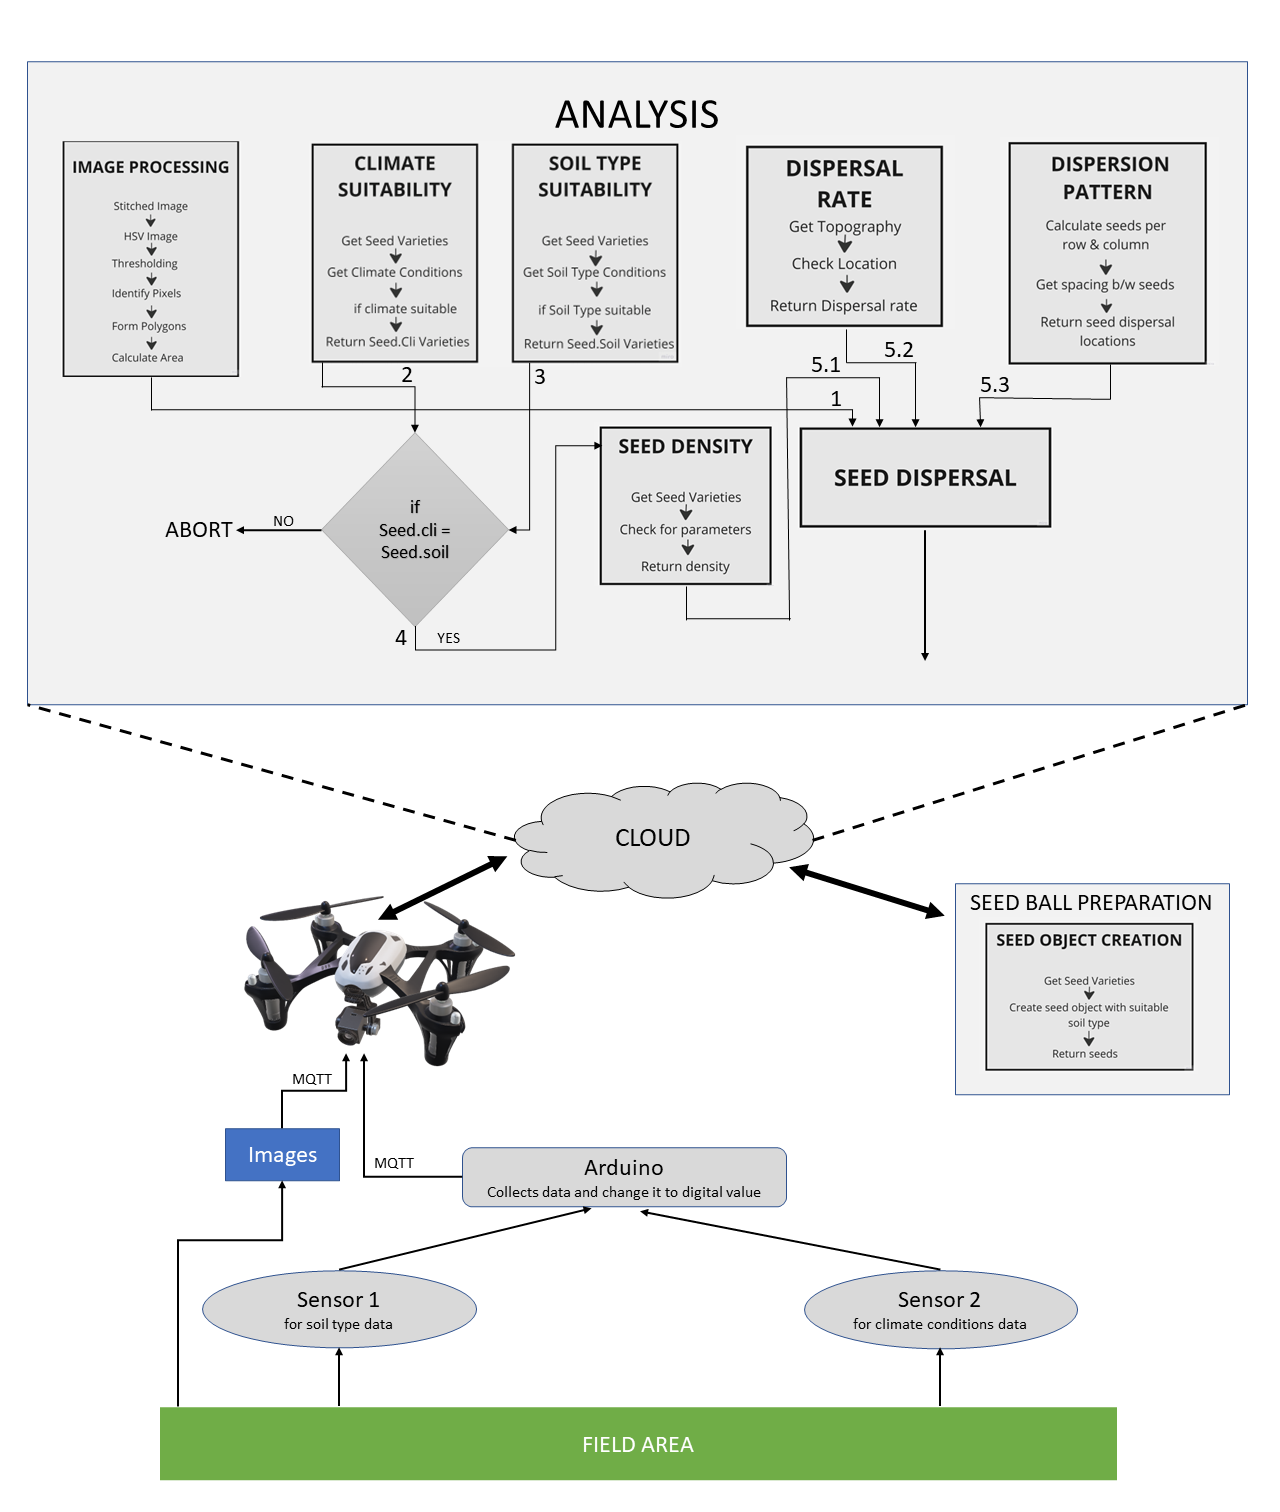
\includegraphics[width=7cm,height=7cm]{architecture_ml.png}
    \caption{SYSTEM ARCHITECTURE}
    \label{sa}
\end{figure}

The architecture for this algorithm can be divided into different modules or stages, each of which performs a specific task. Here's a proposed architecture for the algorithm:
\begin{enumerate}
\item Image Processing Module: This module takes the list of captured images as input, stitches them together into a single image, and converts the image to the HSV colour space. It then applies a color threshold to identify pixels within the range of barren land color and then it forms a polygon with pixels identified and calculates the total area of the polygon formed of barren land.

\item Climate and Soil Suitability Module: This module checks if the climate conditions and soil type are suitable for the selected seed variety. It returns a message indicating whether the climate and soil type is suitable or not.

\item Seed Density Module: This module takes the climate conditions, topography, soil type, and seed variety as input and looks up the recommended seed density for the given seed variety based on the current growing conditions. It returns the recommended seed density as the optimal number of seeds per unit area.

\item Dispersion Pattern Module: This module takes in the location where the seeds need to be dispersed and the total number of seeds as input. It determines the number of seeds to place in each row and column, determines the spacing between each seed, and returns a list of tuples containing the location of each seed along with its associated seed.

\item Seed Object Creation Module: This module takes in the soil type and seed variety as input, creates a seed object with the necessary properties such as water level, nutrient level, etc., and returns the seed object.

\item Seed Dispersal Rate Module: This module takes in the topography and location as input, determines the optimal seed dispersal rate of seeds based on the topography and location, and returns the dispersal rate.

\item Seed Dispersal Module: This module dispatches the drone to the location and begins seed dispersal. It checks whether the seed dispersal was successful or not and returns a message indicating the success or failure of the seed dispersal.
\end{enumerate}


\subsection{Stages of Seed Dispersal}
In this subsection, we discuss the stages of seed dispersal. A sophisticated and effective seed dispersal strategy contains the following stages of seed dispersal:
\begin{enumerate}
\item Aerial Survey \& Mapping: Drones are used to survey and map the terrain to identify places needing plantation. We use hyper-spectral image technology with Machine learning to generate a topographical map to give a holistic sense of the total area.

\item  Understanding The Requirements: Determine trees to be grown based on various parameters like weather, altitude, soil, indigenous seed varieties, and historical growth data using previous information and machine learning.

\item  Seed Balls Preparation: Seed balls are then created as per local soil requirements to ensure safety and no change of direction by the wind.

\item Drone Deployment: Drones are deployed to spray seeds over designated areas. We fly the drones along a pre-determined flight map. These maps are digitally rendered to cover all the areas determined in Step 1 with a topographical overlay for easy visualization.

\item Geo-tagging Drone path: The paths followed by the drones are geo-tagged, facilitating periodic drone monitoring\cite{8} of the sown area to collect tree statistics.

\item Post Growth Monitoring: Geo-tagged seed balls are monitored for growth for years to come to create analytics required for forest monitoring.
\end{enumerate}

The stages of the seed dispersal are shown in Fig. \ref{sd}
\begin{figure}[htp]
    \centering
    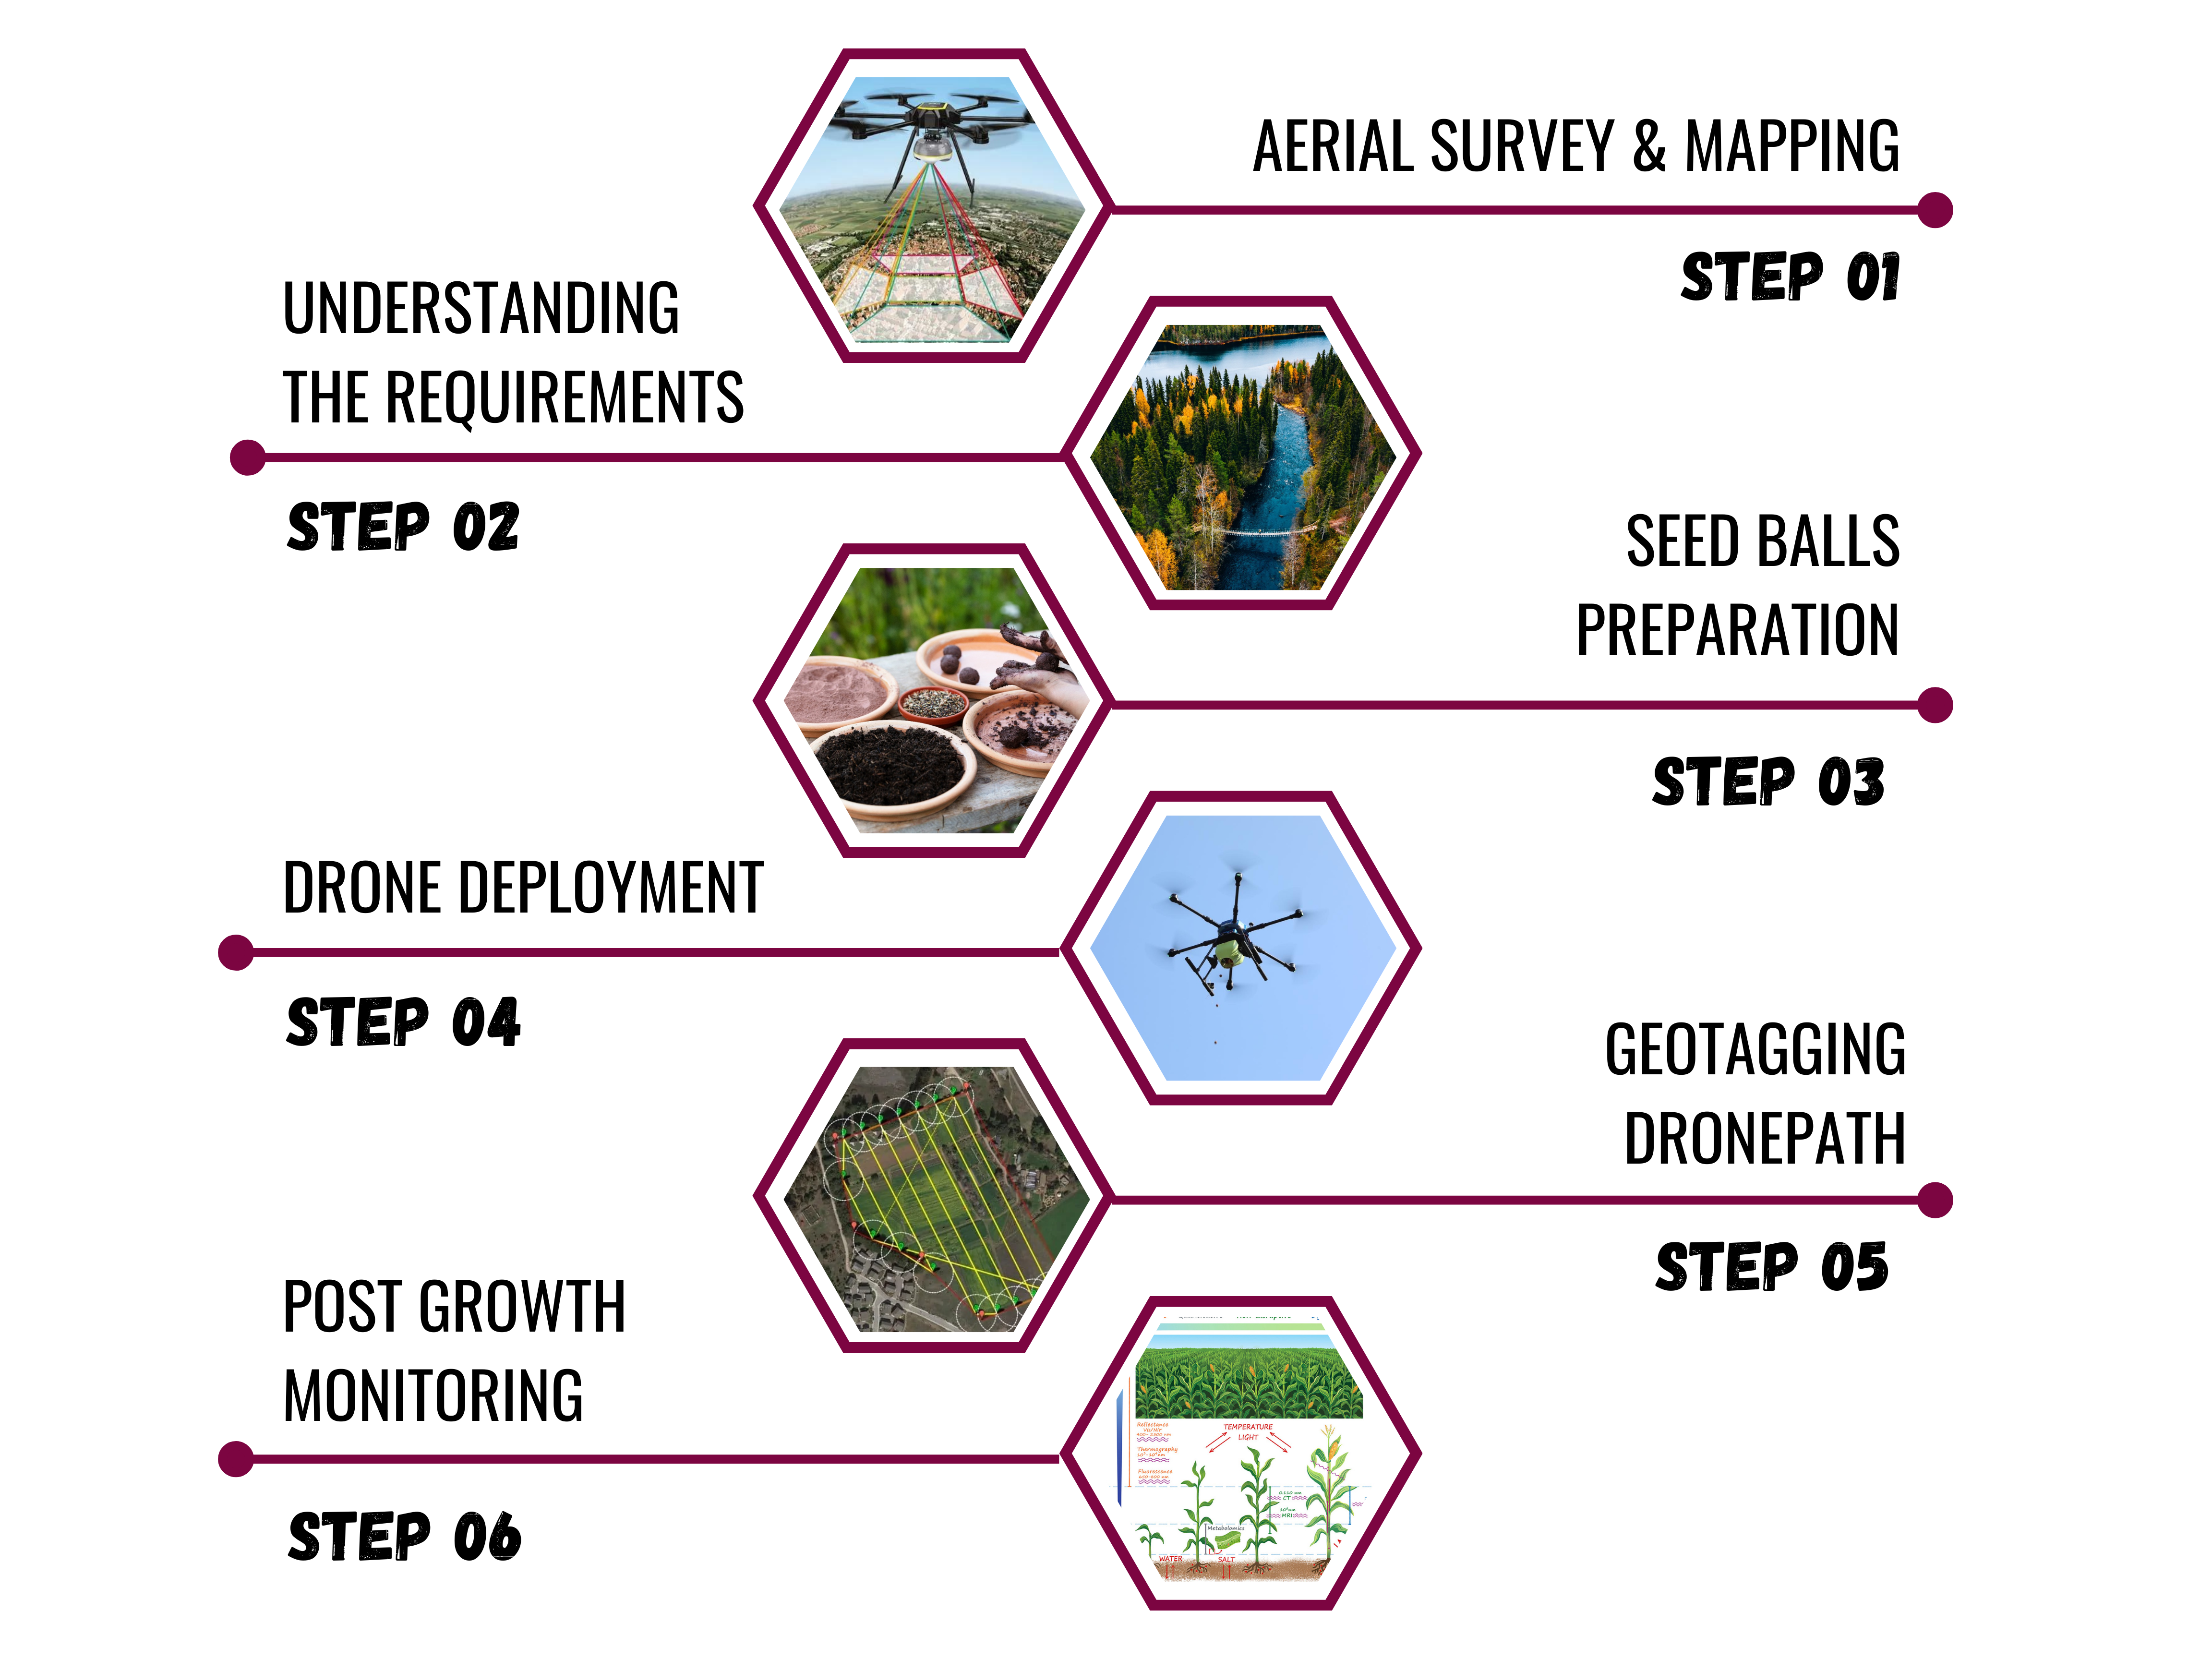
\includegraphics[scale =0.05]{Narcondam_flowchart.png}
    \caption{STAGES OF SEED DISPERSAL}
    \label{sd}
\end{figure}


\subsection{Dispatching mechanism}

Seed dispersal by drones typically involves using a variety of dispatching mechanisms to release and distribute seeds in a target area\cite{7}. Some possible dispatching mechanisms for seed dispersal by drones include the Drop mechanism, Spray mechanism, Pneumatic mechanism, and Glue mechanism. In addition to these mechanisms, drones may also be equipped with sensors and software to help guide seed distribution and optimize the dispersal pattern. For example, drones may use GPS technology to accurately target specific areas avoid sensitive habitats, or use machine learning algorithms to adapt to changing wind conditions or terrain.
\\Drop mechanism is used in this study. Seed dispersal by drones using the dropping mechanism involves releasing the seeds from a container mounted on the drone at a specific location. The container may have a small opening or be designed to open automatically when triggered by the drone's software. The drone may hover or fly over the target area and drop the seeds in a pattern determined by the operator or software. The drone may move or rotate as needed to ensure that the seeds are distributed evenly. One advantage of the dropping mechanism is that it can be used to target specific areas with greater accuracy than other dispersal methods. The operator can control the height and speed of the drone to ensure that the seeds are dropped in the desired location. Additionally, the dropping mechanism can be used to release a wide variety of seed sizes and shapes, making it a versatile option for seed dispersal by drones. Overall, seed dispersal by drones using the drop mechanism is a precise and efficient method that can be used to target specific areas with accuracy.
\\A drone dispatching the seeds in barren land and development of the land  is shown in Fig. \ref{dis}

\begin{figure}[htp]
    \centering
    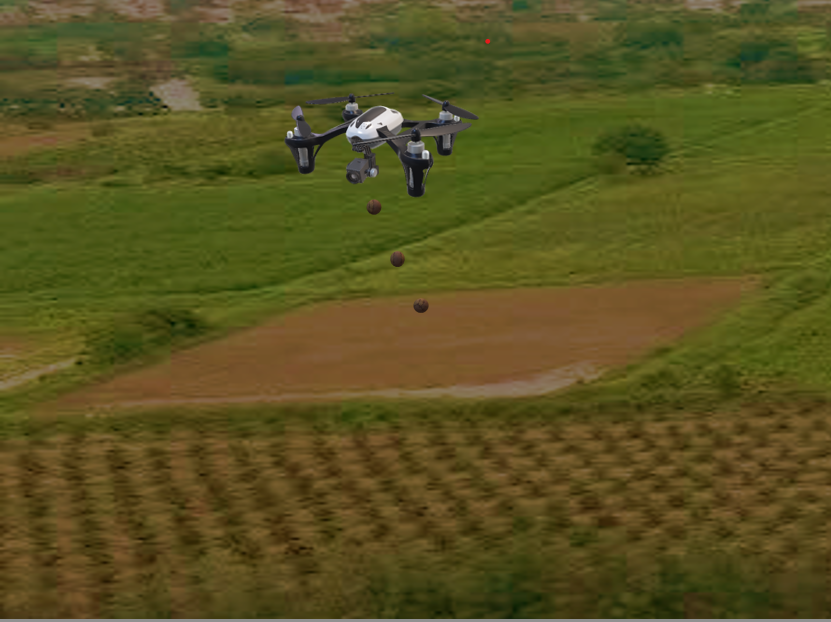
\includegraphics[scale = 0.3]{narcondam.png}
    \caption{DRONE DISPATCHING SEEDS}
    \label{dis}
\end{figure}


\section{Narcondam Hornbill Algorithm}
The Algorithm with different modules and its details are given in brief in Algorithm1.
\newline The Algorithm2 indicates the calling of the main function using the modules of Algorithm1.
\begin{algorithm} [ht]
\begin{scriptsize}
\begin{algorithmic}[1]
\label{algo1}
% \STATE Begin
\STATE \textbf{AIM: Declaring functions which will be called in the main function}
\STATE \textbf{find\_barren\_land\_and\_its\_area}(images) 
    \begin{ALC@g}
    \STATE  Stitched\_image $\gets$ stitch(images)
    \STATE  hsv\_image $\gets$ Stitched\_image
    \STATE  Threshold\_image $\gets$ inRange(hsv\_image, lower\_barren, upper\_barren)
    \STATE  contours $\gets$ findContours(Threshold\_image)
    \FOR{contour in contours}
        \STATE  polygon $\gets$ approxPoly(contour, arcLength)
        \STATE  polygons.append(polygon)
    \ENDFOR
    \STATE  area $\gets$ 0
    \FOR{polygon in polygons}
    \STATE  area $\gets$ area + contourArea(polygon)
    \ENDFOR
    \RETURN  area
    \end{ALC@g}
\smallbreak
\STATE \textbf{is\_climate\_suitable}(climate, seed\_variety)
    \begin{ALC@g}
    \STATE Suitable\_climate $\gets$ read.dataset[]
    \STATE climate\_Suitable$\gets$Suitable\_climate.get(seed\_variety)
    \IF{climate in climate\_Suitable}
        \RETURN  True
    \ELSE
        \RETURN  False
    \ENDIF
    \end{ALC@g}
\smallbreak
\STATE \textbf{is\_soil\_type\_suitable}(soil\_type, seed\_variety)
    \begin{ALC@g}
    \STATE suitable\_soil\_types $\gets$ read.dataset[]
    \STATE Suitable\_types$\gets$suitable\_soil\_types.get(seed\_variety)
    \IF{soil\_type in Suitable\_types}
        \RETURN  True
    \ELSE
       \RETURN  False
    \ENDIF
    \end{ALC@g}
\smallbreak

\STATE \textbf{get\_optimal\_seeds\_per\_unit\_area}(climate,topography,\\soil\_type,seed\_variety) 
    \begin{ALC@g}
    \STATE  density$\gets$Suitable\_densities.get(seed\_variety,climate,\\topography,soil\_type)
    \RETURN  density
    \end{ALC@g}
\smallbreak

\STATE\textbf{disperse\_seeds}(location, total\_seeds)
    \begin{ALC@g}
    \FOR{$i$ \textbf{in range}($seeds\_per\_row$)}
        \FOR{$j$ \textbf{in range}($seeds\_per\_col$)}
            \STATE $x \gets get.disperse\_point\_x(init\_loc, x\_spacing)$
            \STATE $y \gets get.disperse\_point\_y(init\_loc, y\_spacing)$
            \STATE $seed \gets create\_seed('default')$
            \STATE $seeds.append((x, y, seed))$
        \ENDFOR
    \ENDFOR
    \RETURN  $seeds$
    \end{ALC@g}
\smallbreak
\STATE\textbf{create\_seed}(soil\_type, seed\_variety)
    \begin{ALC@g}
    \RETURN  $seed$
    \end{ALC@g}
\smallbreak

\STATE\textbf{determine\_dispersal\_rate}(topography, location)
    \begin{ALC@g}
    \RETURN  $dispersal\_rate$
    \end{ALC@g}
\smallbreak

\STATE\textbf{dispatch\_drone}(location, dispersal\_rate)
    \begin{ALC@g}
    \STATE $drone.takeoff()$
    \STATE $seeds\_dispensed \gets 0$
    \WHILE{$seeds\_dispensed < dispersal\_rate$}
        \STATE $seeds\_dispensed += drone.dispense\_seed()$
    \ENDWHILE
    \STATE $drone.land()$
    \end{ALC@g}


    
\end{algorithmic}
\caption{Narcondam Hornbill Algorithm}
\end{scriptsize}
\end{algorithm}



\begin{algorithm} [ht]
\begin{scriptsize}
\begin{algorithmic}[1]
\STATE \textbf{INPUT}:$A$ $set$ $of$ $images$ $of$ $an$ $area$.
\STATE \textit{\textbf{Training data}}: $dataset$ $for$ $climate$ $type,$ $soil$ $type,$ $seed$ $variety$ $and$ $topography.$
\STATE \textit{\textbf{Testing data}}: $A$ $set$ $of$ $images$ $of$ $field$ $area.$
\STATE \textbf{OUTPUT}: $Whether$ $seeds$ $are$ $dispersed$ $or$ $not.$ 
\medbreak

\STATE \textbf{seed\_dispersal}
(images, climate, topography,\\soil\_type,seed\_variety, location) 
    \begin{ALC@g}
    \STATE {is\_climate\_suitable}(climate, seed\_variety)
    \STATE {is\_soil\_type\_suitable}(soil\_type, seed\_variety)
    \STATE  seeds\_per\_unit\_area $\gets$ {get\_optimal\_seeds\_per\_unit\_area}\\(climate,topography,soil\_type,seed\_variety)
    \STATE  area $\gets$ {find\_barren\_land\_and\_its\_area}(images)
    \STATE  total\_seeds = area*seeds\_per\_unit\_area
    \STATE{disperse\_seeds}(location, total\_seeds)
    \STATE  seed\_dispersal\_location.append(location)
    \STATE  success = {dispatch\_drone}(location, dispersal\_rate)
    \IF{(success)}
        \RETURN   "seed dispersal successful".
    \ELSE
        \RETURN   "seed dispersal failed".
    \ENDIF
    \end{ALC@g}
    
\end{algorithmic}
\caption{Main Function}
\end{scriptsize}
\label{algo:resuti}
\end{algorithm}

 This algorithm takes in a list of images which are captured by the drone during the aerial survey as input, stitches them together into a single image, converts the image to the HSV colour space, applies a colour threshold to identify pixels within the range of barren land colour, and then calculates the total area of the barren land in the image and returns the area of the barren land as output. The algorithm then starts checking if the climate conditions are suitable for the selected seed variety. If the climate is suitable, the algorithm returns a message indicating that the climate is suitable for the selected seed variety. The algorithm also checks if the soil type is appropriate for the selected seed variety. If the soil type is suitable, the algorithm returns a message indicating that the soil type is suitable for the selected seed variety. Next, the algorithm takes in the climate conditions, topography, soil type, and seed variety as input looks up the recommended seed density for the given seed variety based on the current growing conditions, and returns the recommended seed density as the optimal number of seeds per unit area. 
\\The algorithm then takes in the location where the seeds need to be dispersed. The total number of seeds as input determines the number of seeds to place in each row and column determines the spacing between each seed, creates a seed object, and returns a list of tuples containing the location of each seed along with its associated seed object. The algorithm then takes in the soil type and seed variety as input creates a seed object with the necessary properties such as water level, nutrient level, etc, and returns the seed object. The algorithm takes in the topography and location as input, determines the optimal seed dispersal rate of seeds based on the topography and location, and returns the dispersal rate. The drone is then dispatched to the location and begins seed dispersal. If the seed dispersal is successful, the algorithm returns a message indicating that the seed dispersal was successful. If the seed dispersal is not successful, the algorithm returns a message indicating that the seed dispersal failed.

\section{Simulation and Results Analysis}
This section discusses the environment setup map, datasets, and simulation results analysis.
\subsection{Simulation}
The proposed architecture can be implemented using various programming languages and frameworks such as Python, OpenCV, NumPy, etc. Each module can be implemented as a separate function or class, and the overall algorithm can be designed as a series of function calls.

\subsubsection*{Dataset}
In this section, we present the dataset used in our seed dispersal algorithm. These data were generated using a random forest Machine Learning Algorithm, that learns patterns and features associated with different seed varieties or climate conditions based on labelled training data. 
The Random Forest algorithm was chosen for its ability to handle complex datasets with high-dimensional features and robustness to overfitting. RF constructs multiple decision trees during training, improving generalization performance. It can handle both numerical and categorical data without extensive preprocessing. It is also less sensitive to outliers and noise and provides variable importance measures for model interpretation. Thus RF was chosen over other machine learning algorithms due to its balance of performance, interpretability, and ease of implementation. The dataset includes information about suitable climates, and soil types for various crops.

The Table \ref{1} shows the suitable climates for different crops:
\begin{table}[h]
  \centering
    \caption{Suitable Climates for Crops}
  \begin{tabular}{|c|c|}
    \hline
    \textbf{Crop} & \textbf{Suitable Climates} \\
    \hline
    Tomato & Hot, Plenty of sunshine \\
    Loki & Cool\_moist, Shade or partial sun \\
    Okra & Cool, Plenty of sunshine \\
    Mirchi & Hot, Plenty of sunshine \\
    Cotton & Cool\_moist, Plenty of sunshine \\
    Corn & Hot, Shade or partial sun \\
    Paddy & Hot, Plenty of sunshine \\
    Melon & Cool\_moist, Shade or partial sun \\
    \hline
  \end{tabular}
  \label{1}
\end{table}
%\subsection{Suitable Soil Types}
The Table \ref{2} shows the suitable soil types for different crops:
\begin{table}[h]
  \centering
    \caption{Suitable Soil Types for Crops}
  \begin{tabular}{|c|c|}
    \hline
    \textbf{Crop} & \textbf{Suitable Soil Types} \\
    \hline
    Tomato & Loam, Sandy loam \\
    Loki & Loam, Clay loam \\
    Okra & Loam, Sandy loam \\
    Mirchi & Loam, Clay loam \\
    Cotton & Loam, Clay loam \\
    Corn & Loam, Sandy loam \\
    Paddy & Loam, Clay loam \\
    Melon & Clay loam, Sandy loam \\
    \hline
  \end{tabular}
  \label{2}
\end{table}

In the proposed algorithm, we have used properties, such as soil type, growth rate, health, water, and nutrient Level

\subsection{Results Analysis}
Fig. \ref{env} shows the environment setup considered to test the proposed algorithm. The proposed algorithm deployed in the drone executes all the stages of seed dispersal discussed in the previous section. The drone-based seed dispersal is shown in Fig. \ref{dis}.
\begin{figure}[htp]
    \centering
    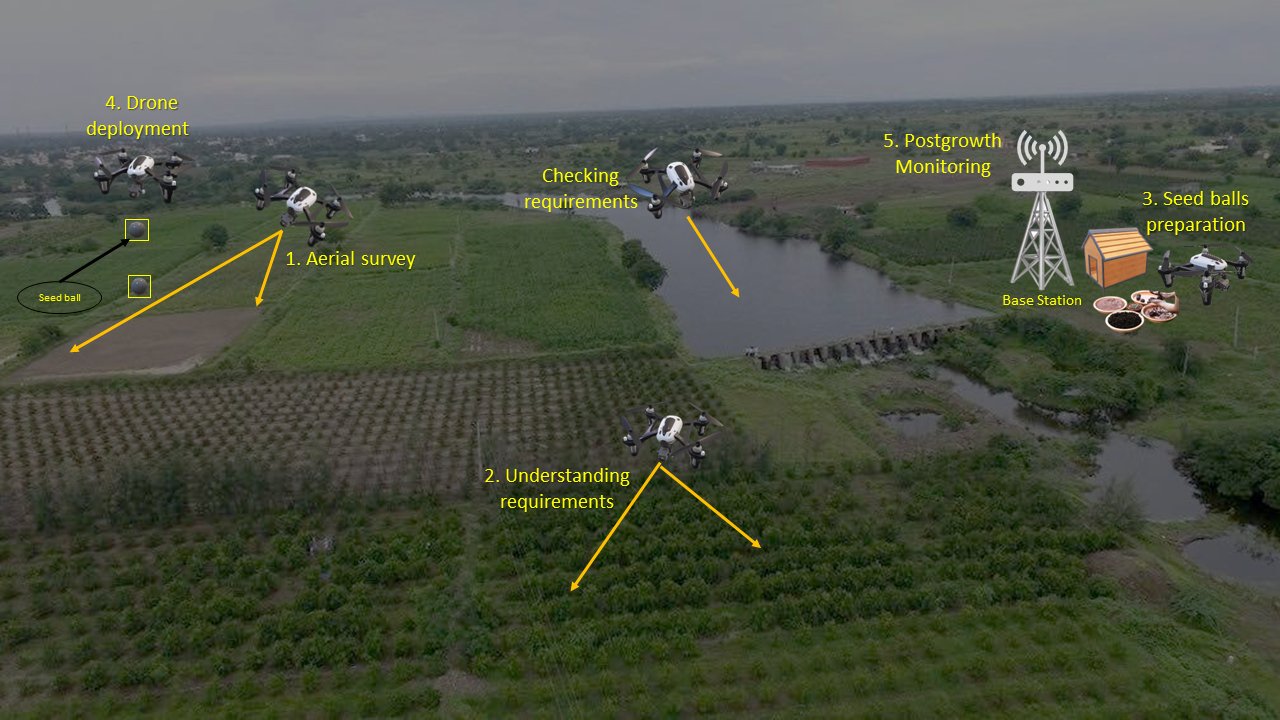
\includegraphics[scale=0.2]{hornbill.png}
    \caption{Environment setup map}
    \label{env}
\end{figure}
%When an unknown environment is given the drone uses our algorithm and performs the seed dispersal. All the stages of seed dispersal are executed one after the other and tested on the given environment as shown in Fig. \ref{env}.
%\section{Simulation and Results Analysis}
%as shown in Fig. \ref{ds}, Fig. \ref{de}, Fig. \ref{df} and Fig. \ref{dt}.
To test the developed algorithm, we have considered the dataset that consists of different suitable climate conditions, recommended seed densities based upon parameters like climate, topography, etc, and soil conditions for a few seed varieties like Tomato, Loki, Okra, Mirchi, etc was used and the results of suggested dispersal rate and soil type suitability were predicted.
We have analyzed the algorithm with parameters such as seed dispersal rate, seed variety, sandy loom soil, clay loom soil, topography, and location (forest or barren land). 
The study focuses on seed dispersal dynamics in complex ecological systems using simulations. The approach assumes that ecological processes can be adequately represented and modeled, including disperser behavior, environmental factors, and landscape structure. Key ecological parameters like seed traits, disperser characteristics, and landscape features are incorporated, based on literature, field observations, and expert knowledge. Spatial and temporal scales are employed to balance computational efficiency with ecological fidelity. Stochasticity and uncertainty are considered, allowing for the robustness and consistency of results. These assumptions guide the modeling approach and interpretation of results, aiming to develop a realistic representation of seed dispersal dynamics.
Seed dispersal rate concerning topography refers to how the distribution and movement of seeds are influenced by the shape and features of the land or terrain. Topography plays a crucial role in determining where seeds will disperse and how far they will travel, which, in turn, affects plant population dynamics and ecosystem diversity. Fig. \ref{ds} shows the variation of dispersal rate concerning different topographical areas.
\begin{figure}[htp]
    \centering
    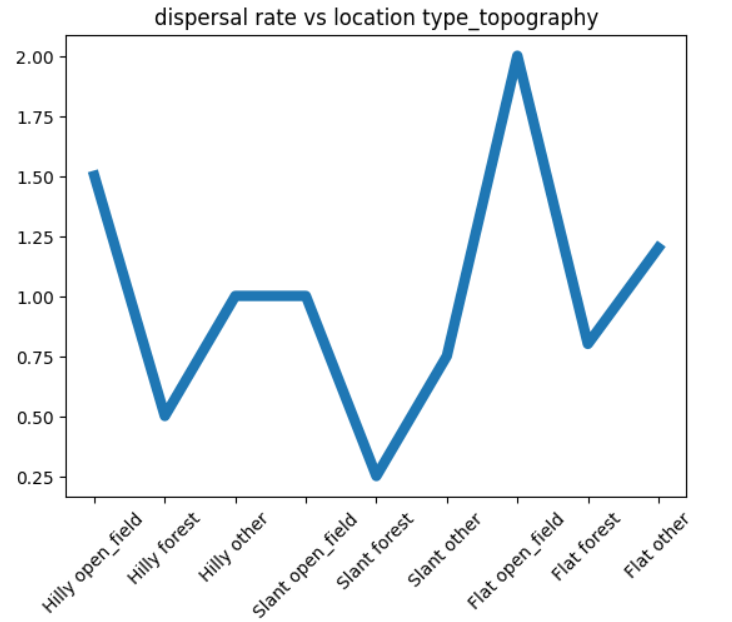
\includegraphics[scale=0.5]{plot11.png}
    \caption{Seed dispersal rate concerning topography}
    \label{ds}
\end{figure}
The results as shown in Fig. \ref{de}, Fig. \ref{df}, and Fig. \ref{dt} show the suitability of different soil conditions for the available seed varieties and thus output whether the soil is suitable or not. In these results, 1 represents suitability and 0 represents unsuitable soil.
Fig. \ref{de} shows the suitability of seed varieties concerning the soil condition - sandy loam.
\begin{figure}[htp]
    \centering
    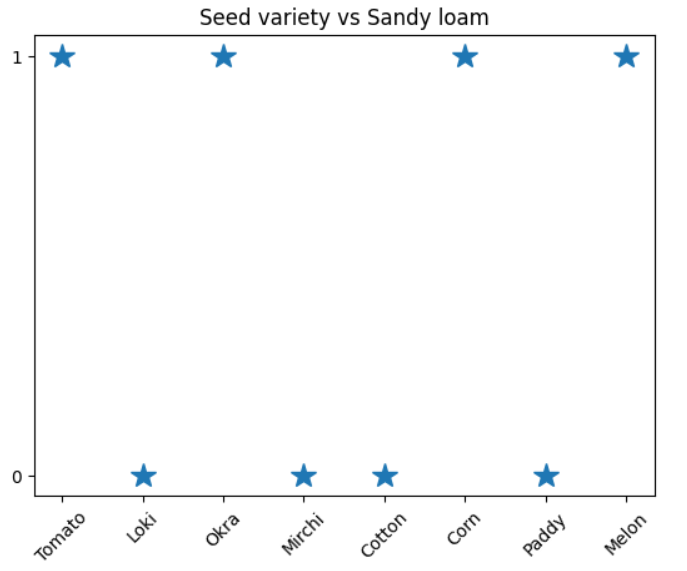
\includegraphics[scale=0.5]{plot12.png}
    \caption{Seed variety concerning sandy loam}
    \label{de}
\end{figure}
Fig. \ref{df} shows the suitability of seed varieties concerning the soil condition - loam.
\begin{figure}[htp]
    \centering
    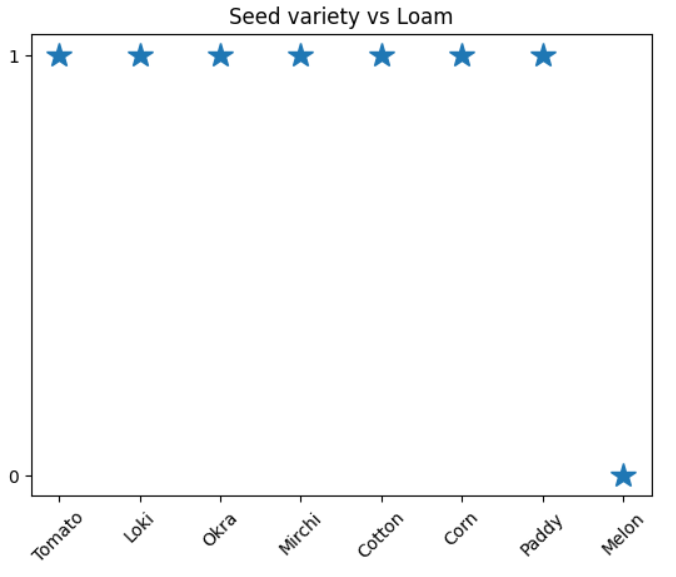
\includegraphics[scale=0.5]{plot13.png}
    \caption{Seed variety concerning loam}
    \label{df}
\end{figure}
Fig. \ref{dt} shows the suitability of seed varieties concerning the soil condition - clay loam.
\begin{figure}[htp]
    \centering
    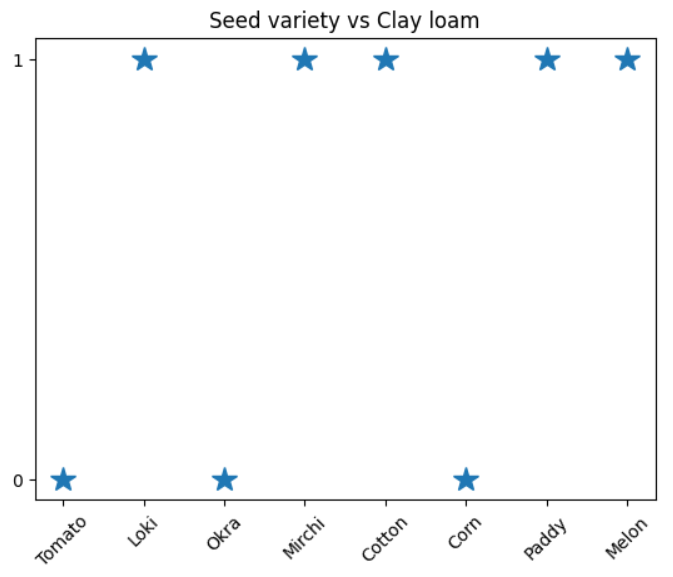
\includegraphics[scale=0.5]{plot14.png}
    \caption{Seed variety concerning clay loam}
    \label{dt}
\end{figure}
\begin{figure}[htp]
    \centering
    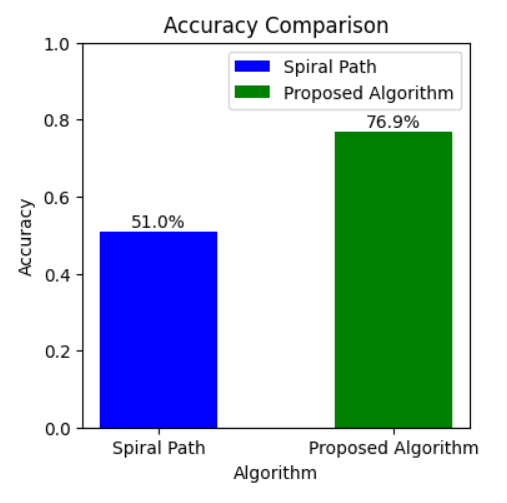
\includegraphics[scale=0.7]{plot15.png}
    \caption{Accuracy comparison}
    \label{dac}
\end{figure}
\begin{figure}[htp]
    \centering
    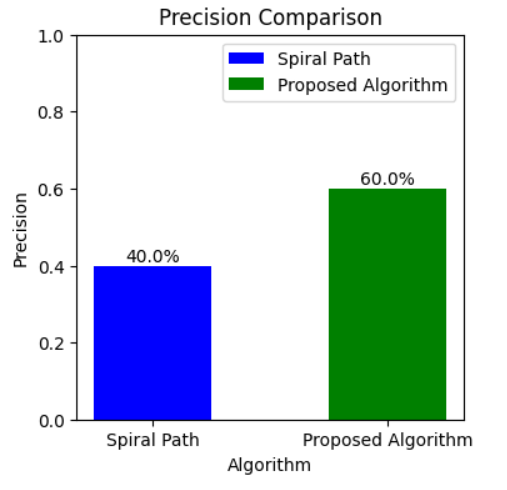
\includegraphics[scale=0.7]{plot16.png}
    \caption{Precision comparison}
    \label{dpr}
\end{figure}
The comparative graphs obtained and shown in Fig. \ref{dac} and Fig. \ref{dpr}, are evident that the proposed algorithm outperforms the existing Spiral Path algorithm \cite{9} significantly. The proposed algorithm significantly outperforms the existing Spiral Path algorithm in terms of accuracy and precision. The algorithm provides more than 0.76 accuracies and 0.6 precision, while the existing Spiral Path algorithm provides 0.51 accuracy and 0.4 precision. The improved performance is attributed to innovative features and optimizations, making it a more advanced and efficient solution for distance-related tasks. The proposed algorithm offers flexibility, accuracy, and scalability. However, addressing challenges related to data requirements, interpretability, generalizability, and mechanistic understanding is essential for advancing the utility and robustness of the proposed approach.

\section{Conclusions and Future Work}
This paper presented a novel Narcondam Hornbill-inspired seed dispersal algorithm for barren lands. We have developed the system architecture and drone-based seed dispersal stages. The proposed algorithm utilized a random forest machine learning algorithm for predicting the seed variety and its rate at a particular location. Finally, we simulated the proposed algorithm in Python, by considering the variety of seeds, soil types, and different climate conditions. In addition, we compared it with the existing seed dispersal algorithm, that is, the Spiral Path Algorithm. The proposed algorithm outperforms as compared to it, with an accuracy of 76.9\% and 60\% precision. This shows the improvement in the seed dispersal efficiency, precision, and accuracy, and also offers more flexibility and scalability. In the future, the algorithm could be further refined and tested in real-world scenarios such as reforestation and conservation efforts.

%In conclusion, the Narcondam Hornbill-inspired seed dispersal algorithm provides a novel approach by simulation of the hornbill's dispersal process and its consideration of environmental factors improves the accuracy and efficiency of the seed dispersal process, improving seed dispersal efficiency and accuracy. The algorithm's ability to optimize the process for different environmental conditions and seed types could have significant benefits for plant species survival and ecosystem biodiversity. The algorithm has the potential to greatly improve the effectiveness of seed dispersal in barren lands and may help to mitigate the effects of environmental degradation. The algorithm offers a more efficient and accurate way of simulating seed dispersal in a simulated environment. future, the algorithm could be further refined and tested in real-world applications such as reforestation and conservation efforts.

\section*{Acknowledgement} The work is supported by the Indian Institute of Information Technology Raichur, Karnataka, India, and is partially funded by the Brazilian National Council for Scientific and Technological Development - CNPq, via Grant No. 306607/2023-9. Ashit Kumar Dutta would like to express sincere gratitude to AlMaarefa University, Riyadh, Saudi Arabia, for providing funding to conduct this research.
\begin{thebibliography}{1}
\bibitem{1} Lohit GV, Bisht D. Seed Dispenser using Drones and Deep Learning Techniques for Reforestation. In2021 5th International Conference on Computing Methodologies and Communication (ICCMC) 2021 Apr 8 (pp. 1275-1283). IEEE.
\bibitem{2}Lakhan A, Elhoseny M, Mohammed MA, Jaber MM. SFDWA: secure and fault-tolerant aware delay optimal workload assignment schemes in edge computing for Internet of drone things applications. Wireless Communications and Mobile Computing. 2022 Feb 25;2022.
\bibitem{3} Nishar, A.; Richards, S.; Breen, D.; Robertson, J.; Breen, B. Thermal infrared imaging of geothermal environments and by an unmanned aerial vehicle (UAV): A case study of the Wairakei – Tauhara geothermal field, Taupo, New Zealand. Renew. Energy 2016, 86, 1256–1264.
\bibitem{4} Naniwadekar R, Ghuman S, Gopal A, Page N, Ramachandran V. Characteristics of Narcondam Hornbill Rhyticeros narcondami nest trees. Hornbill Natural History and Conservation. 2020;1:1-9.
\bibitem{5}Naniwadekar R, Ghuman S, Gopal A, Page N, Ramachandran V. Characteristics of Narcondam Hornbill Rhyticeros narcondami nest trees. Hornbill Natural History and Conservation. 2020;1:1-9.
\bibitem{6}Manchi S. Status, ecology and conservation of Narcondam Hornbill Aceros narcondami on the Narcondam Island, India. Salim Ali Centre for Ornithology and Natural History. 2017.
\bibitem{7}Marzuki OF, Teo EY, Rafie AS. The mechanism of drone seeding technology: a review. Malays. For. 2021 Jun;84:349-58.
\bibitem{8}Mohammed MA, Lakhan A, Abdulkareem KH, Abd Ghani MK, Marhoon HA, Nedoma J, Martinek R. Multi-objectives reinforcement federated learning blockchain-enabled Internet of things and Fog-Cloud infrastructure for transport data. Heliyon. 2023 Nov 1;9(11).
\bibitem{9} Tamura K, Yasuda K. Primary study of spiral dynamics inspired optimization. IEEJ Transactions on electrical and electronic engineering. 2011;6(S1):S98-100.
\end{thebibliography}
\end{document}




